% Technische Universität Dresden
% Fakultät Informatik
% Institut für Software- und Multimediatechnik
% Seniorprofessur für Multimediatechnik
%
% Example document demonstrating the usage of mmthesis.sty
% 2012-10-26 Andreas Rümpel
% 
% ### build hints (% = filename of tex file) ###
% pdflatex: pdflatex %.tex
% biber: biber % (biber is a modern backend for bibtex, http://biblatex-biber.sourceforge.net)
% glossaries and acronyms: makeglossaries %
%
% Das LATEX2e-Sündenregister: ftp://ftp.dante.de/tex-archive/info/l2tabu/german/l2tabu.pdf
% KOMAScript-Guide: ftp://ftp.dante.de/tex-archive/macros/latex/contrib/koma-script/scrguide.pdf
% Einige typographische Grundregeln und ihre Umsetzung in LaTeX: http://www2.informatik.hu-berlin.de/sv/lehre/typographie.pdf

\documentclass[
	headsepline,
	footsepline,
	fontsize=12pt,
	%draft, % use this for finding overfull boxes
	%parskip, % use this for alternative paragraph formatting
	bibliography=totoc
]{scrbook}


\usepackage[utf8]{inputenc}
\usepackage{mmthesis}
\addbibresource{library.bib} % put name of bib file here with extension

%### switches
%\printoutput % make link colors black, leave deactivated for screen output

%### define metadata
\mmtype{Diplomarbeit} %Diplomarbeit|Großer Beleg|Bachelorarbeit|Masterarbeit|Seminararbeit
\mmtitle{Semantik-gestütztes Hilfesystem für ein komposites Informationsvisualisierungssystem}
\mmtshorttitle{Hilfesystem für komposite InfoVis}
\mmtauthor{Nikolaus Piccolotto}
\mmtsubmissionmonth{November 2013}
\mmtsubmissiondate{30. November 2013}
\mmtsupervisor{Dipl.-Medieninf. Martin Voigt}
%\mmtsupervisorii{Dipl.-Medieninf. Foo Bar} % Co-supervisor, optional

\mmthypersetup % has to be called after setting metadata

%### acronyms
\newacronym{PDF}{PDF}{Portable Document Format}
\newacronym{RCP}{RCP}{Rich Client Platform}
\newacronym{RIA}{RIA}{Rich Internet Application}
\newacronym{RELAXNG}{RELAX NG}{Regular Language Description for XML New Generation}
\newacronym{SGML}{SGML}{Standard Generalized Markup Language}
\newacronym{SWT}{SWT}{Standard Widget Toolkit}
\newacronym{WDC}{W3C}{World Wide Web Consortium}
\newacronym{WPF}{WPF}{Windows Presentation Foundation}
\newacronym{XPath}{XPath}{XML Path Language}
\newacronym{XHTML}{XHTML}{Extensible Hypertext Markup Language}
\newacronym{XML}{XML}{Extensible Markup Language}


\begin{document}
\frontmatter
\pagenumbering{Roman}
\mmtfrontmatter

\listoffigures
\listoftables
\printglossary[type=\acronymtype,style=long,title=Abkürzungsverzeichnis,toctitle=Abkürzungsverzeichnis]
%\printglossary %Glossar

\mainmatter

\chapter{Einleitung}
\label{chapter:einleitung}

% Hier kommt eine kurze Einführung von semantischen Daten, nehme ich an

\section{Motivation}
\label{section:motivation}

% Hier wird generell eingeleitet, also vermutlich die Problematik zwischen semantischen Datensätzen und Endusern

\section{Problemstellung und Zielsetzung}
\label{section:problemstellung}

% Hier wird quasi der Vizboard Workflow umrissen
% und erklärt, wo das eigentliche Problem liegt, nämlich im Information Overload beim letzten Schritt

\begin{figure}[htbp]
	\centering
	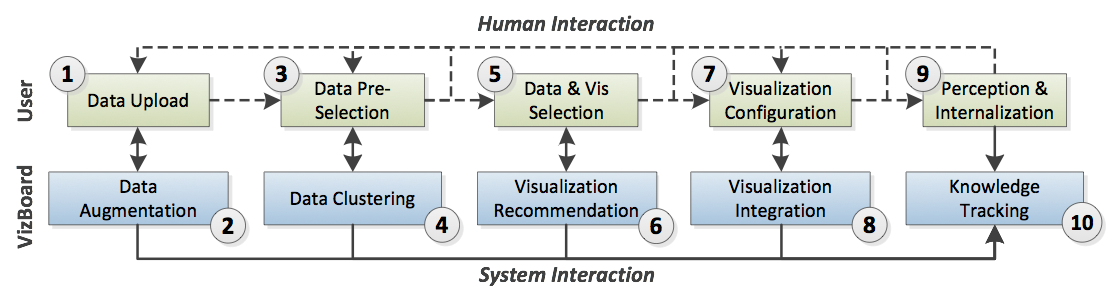
\includegraphics[width=0.75\textwidth]{images/vizboard_workflow.png}
	\caption{VizBoard Workflow}
	\label{figure:vizboard_workflow}
\end{figure}

\section{Aufbau der Arbeit}
\label{section:aufbau}

% Aufbau der Arbeit erklären, kommt zum Schluss


%### end of appendix
%#####################################################
\printbibliography[title=Literaturverzeichnis]

%\printindex

\end{document}